% Sample file on how to use subfiles.
\documentclass[ExampleMasters.tex]{subfiles}

\begin{document}
\clearpage


\chapter{Fault detection and system ability (5 Seiten)}
\label{chap:fault_detection}
\section{Failure Mode and Effects Analysis (FMEA)}
\label{sec:FMEA}
FMEAs were first used by NASA in the apollo project in the 1960s.
A FMEA is used to detect possible failures before they appear. Therefore the FMEA is done in a early stage of a project in order to be able to take the results of the FMEA into consideration when developing a system. In the process every possible failure of a system are taken into consideration. 

In a first step a block diagram of the system with all of its inputs, outputs and subsytems was created to gain a complete understanding of the system. Every subsystem was broken down to the lowest level and for those subsystems block diagrams with all the components, inputs and outputs were created as well.

Starting from the block diagrams all potential failure modes were determined for every component of the system respectively subsystem. As a next step the potential effects of these failure modes were determined and the severity of these effects were evaluated on a scale from one to ten,  with 1 being the lowest severity and ten being the highest severity. For the evaluation a table that shows how different severities correlate with the numbers was used (see Table \ref{tab:fmea_severity}). 
Following this, potential causes for every failure mode were defined. Then the probability of occurrence for each cause was evaluated, also using a scale from one to ten (Table \ref{tab:fmea_probability}).
After that the current control mechanisms, that detect the failure when it should appear, were listed for each failure mechanism and the detectability of the failure mechanism was evaluated using a scale from one to ten (Table \ref{tab:fmea_detectability}).
After the severity, probability and detectability were evaluated, a risk priority number is calculated as follows: 
\begin{equation*}
RPN=severity*probability*detectability
\end{equation*}      
This risk priority number is used to identify the failure mechanisms that need to be addressed. In table \ref{tab:RPN} it is shown how the risk priority number have to be handled.
\begin{table}[h]
	\centering
	\caption{Risk priority number}
	\label{tab:RPN}
	\begin{tabular}{l|l|}
		RPN   & Action  \\ \hline
		0$<$RPN$<$40     &       No action needed           \\
		40$<$RPN$<$100   &      Decide if action is needed after review      \\
		RPN$>$100 &      Action needed         \\
		
	\end{tabular} \\
\end{table}
For the failure mechanisms that need to be addressed actions were decided, that either lower the severity, probability or detectability of them or more than one of those factors. After the performance of these actions the severity, probability and detectability were evaluated again and a new RPN was calculated. If the RPN still is to high a iteration of the process was done.
Figure \ref{fig:fmea_example} shows a screen shot of the FMEA-Excel-worksheet for the first iteration.    
\begin{figure}[h]
	\centering
	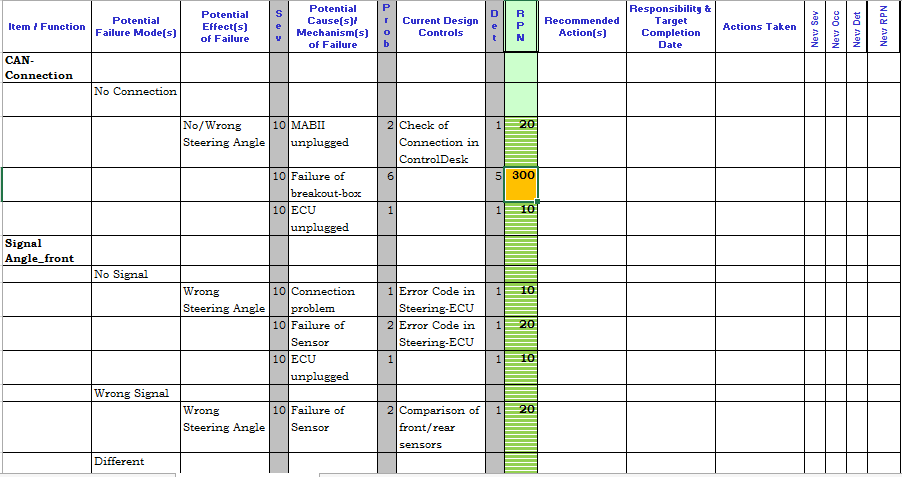
\includegraphics[width=1.0\linewidth]{figures/fmea_example}
	\caption[]{Example of FMEA-worksheet for the first step of the FMEA}
	\label{fig:fmea_example}
\end{figure}

\section{Safety concepts}
\label{sec:safetyconcepts}

\section{Maximum capabilities of the system}
\label{sec:maxi_capabilities}
The capabilities of the system can be divided into two parts. For one thing there are the capabilities that are independent from influences. These are the maximum steering angle and maximum steering rate, which is limited through the ETS-ECU, because of the physical limitation of the hydraulic system.
For another thing there are the capabilities that are influenced by the vehicle speed, load of the dolly, state of the hydraulic and electrical system of the dolly, and environmental influences.
Depending on those parameters the capabilities are lowered.
\begin{itemize}
	\item give indicator of maximum angle/angle rate
	\item describe "algorithm"/lookuptable
	\item explain underlying physical correlation (ref to MA from )
\end{itemize}

\section{Warning and state-info system}
\label{sec:warning_system}
\begin{itemize}
	\item warnings from dolly ECU \\
	In the original state, the ETS-ECU monitors all safety critical components of the dolly. In case of a malfunction, an error code is sent via the CAN-Bus and the error message is visible on the diagnose displays of the dolly. Depending on the severity of the error the steering is deactivated and the axes steer back to a steering angle of 0 deg.
	Due to the required modification of the ASF- and speed-signal, the inbuilt supervision of the ETS-ECU is no longer fully functioning. Therefore a additional supervision of the system has to be implemented in the Simulink-model. This supervision considers the current capabilities of the dolly and reduces the requested steering angle or steering rate, if needed.    
	\item warnings from EBS
	\item warnings from vehicle
	\item 'own' error codes and warnings (e.g. logging, MABII related, arduino-IMU related)
\end{itemize}




\end{document}
